\documentclass{article}
\usepackage{pgfplots}
\pgfplotsset{compat=1.18}
\usepgfplotslibrary{fillbetween}

\begin{document}

The area between $f(x) = \sqrt{x}$ and $g(x) = x^2$ on $[0,1]$ is $1/3$.

\begin{figure}[h]
\centering
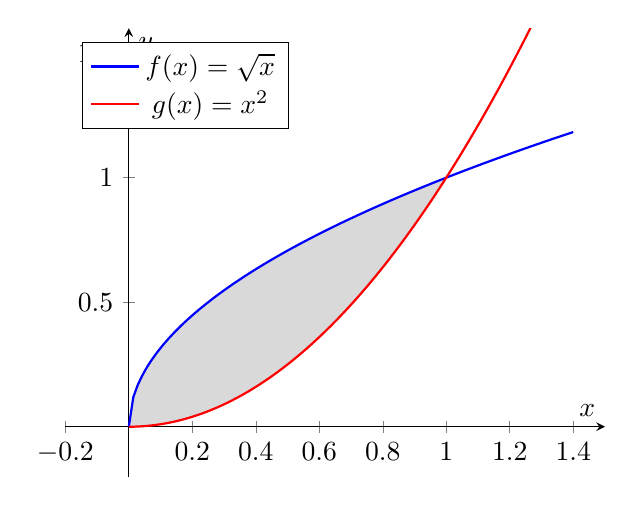
\begin{tikzpicture}
\begin{axis}[
    axis lines=middle,
    xlabel={$x$},
    ylabel={$y$},
    xmin=-0.2, xmax=1.5,
    ymin=-0.2, ymax=1.6,
    samples=100,
    domain=0:1.4,
    legend pos=north west,
]
\addplot[name path=f, blue, thick] {sqrt(x)};
\addlegendentry{$f(x)=\sqrt{x}$}
\addplot[name path=g, red, thick] {x^2};
\addlegendentry{$g(x)=x^2$}
\addplot[gray!30] fill between[of=f and g, soft clip={domain=0:1}];
\end{axis}
\end{tikzpicture}
\caption{The region between two curves.}
\end{figure}

\begin{figure}[h]
\centering
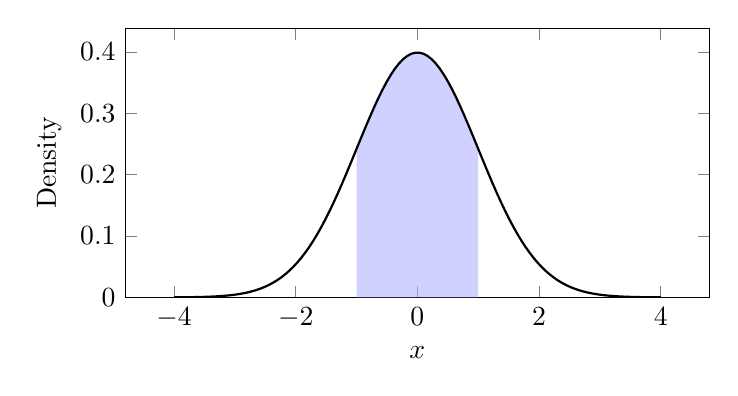
\begin{tikzpicture}
\begin{axis}[
    xlabel={$x$}, ylabel={Density},
    domain=-4:4, samples=120,
    ymin=0, height=5cm, width=9cm,
]
\addplot[name path=pdf, thick, black] {exp(-x^2/2)/sqrt(2*pi)};
\path[name path=axis] (axis cs:-4,0) -- (axis cs:4,0);
\addplot[blue!30, opacity=0.6] fill between[of=pdf and axis, soft clip={domain=-1:1}];
\end{axis}
\end{tikzpicture}
\caption{About 68\% of a normal distribution lies within one standard deviation.}
\end{figure}

\end{document}
